% FEUP THESIS STYLE for LaTeX2e
% how to use feupteses (changed from the original for MIEEC)
%
% FEUP, JCL & JCF, Tue May 20 18:53:15 2008
%
% PLEASE send improvements to jlopes at fe.up.pt, jcf at fe.up.pt
%

%%========================================
%% Commands: pdflatex mieic
%%           bibtex mieic
%%           makeindex mieic (only if crating an index) 
%%           pdflatex mieic
%%========================================

%% For one side layout comment next line and uncomment the second line
\documentclass[11pt,a4paper,twoside,openright]{report}
%\documentclass[11pt,a4paper]{report}

%% For iso-8859-1 (latin1), comment next line and uncomment the second line
\usepackage[utf8]{inputenc}
%\usepackage[latin1]{inputenc}

%% Use option portuges if needed
\usepackage[english]{babel}

%% For the final version, comment next line and uncomment the second line
\usepackage{mieic-distrib/feupteses}
%\usepackage[alpharefs]{feupteses} 

\RequirePackage[round]{natbib}

%% Options: 
%% - portuges: titles, etc in portuguese
%% - provisional: the thesis has not been approved yet
%% - usewatermark: use watermark instaed of provisonal text
%% - print: links are not shown (for paper versions)
%% - alpharefs: bibliography references are alphabetic
%% - numericrefs: bibliography references are numbered (in order of citation)
%% ( by default: author-date format of the ``natbib'' package is used 
%%   the portuguese version requires the file ``plainnat-pt.bst'' to be 
%%   present in the same directory )

%% Include MIEIC definitions different from standard style
\usepackage{mieic-distrib/mieicpatch}

%% Provide a version number in order to keep track of
%% thesis versions (it will printed in the footer of most pages)

\version{NaN}

%% Uncomment in the final version in order to make version footer disappear
\noversiontrue                 

%% Uncomment to create an index (at the end of the document)
%\makeindex                      

%% Path to the figures directory
%% TIP: use folder ``figures'' to keep all your figures
\graphicspath{{figures/}}       

%%----------------------------------------
%% TIP: if you want to define more macros, use an external file to
%% keep them
%some macro definitions

% format
\newcommand{\class}[1]{{\normalfont\slshape #1\/}}

% entities
\newcommand{\Feup}{Faculdade de Engenharia da Universidade do Porto}

\newcommand{\svg}{\class{SVG}}
\newcommand{\scada}{\class{SCADA}}
\newcommand{\scadadms}{\class{SCADA/DMS}}

%%----------------------------------------

%%========================================
%% Start of document
%%========================================
\begin{document}

%%----------------------------------------
%% Information about the work
%%----------------------------------------
\title{Novelty Detection for Visual Place Classification \\ \large{Technical Report}}
\author{André Susano Pinto}
\degree{Master in Informatics and Computing Engineering}
%% Date of submission
%\thesisdate{17$^{th}$ June, 2011}

%% Insert copyright text if used
%\copyrightnotice{Name of the Author, 2008}

\supervisor{Supervisor}{Luis Paulo Reis}{(Dr.)}
\supervisor{Second Supervisor}{Andrzej Pronobis}{(Mr.)}

%% Uncomment committee stuff in the final version
\committeetext{Approved in oral examination by the committee:}
\committeemember{Chair}{Name of the President}{(Title)}
\committeemember{External Examiner}{Name of the Examiner}{(Title)}
\committeemember{Supervisor}{Name of the Supervisor}{(Title)}
\signature
\committeedate{31$^{st}$ July, 2011}

%% Specify cover logo (in folder ``figures'')
\logo{feup-logo.pdf}

%%----------------------------------------
%% Cover page(s)
%%----------------------------------------
\maketitle

%% Uncomment next line in the final version
%\committeepage
%MIEEC uses an external PDF page with the signatures (juri.pdf)
%\includepdf[pagecommand={},noautoscale=false,fitpaper=true,pages=-]{juri.pdf}

%% Preliminary materials
\StartPrelim
\begin{singlespace}
  \chapter*{Abstract}

This should probably be written as last thing.

\chapter*{Resumo}
Let $E$ denote the set of all possible texts in English and $P$ the set of
all possible texts in Portuguese. A transformation $T_{E->P}(x)$ can be defined
in $E \times P$, such that it maps $x \in E$ to a translated version $y \in P$ such
that they hold the same semantic meaning to a reader.

Assume this text to be $T_{E->P}(abstract)$.
\footnote{What I mean is that this will be a translation of the english text present
on abstract and don't expect it to be filled in before the final version of this
document!}

 % the abstract
  %\chapter*{Acknowledgements}
This thesis would have not been possible without the help of some other persons.
I would like to thank to Andrzej Pronobis, for introducing me to the problem and
directing it towards my interests in computer science, for the meetings, insights
and endless reviews of my work. Also to Carl Henrik Ek, for enthusiastically taking part
on the meetings discussing graphical models and related work.

The Computer Vision and Active Perception Lab at Royal Institute of Technology
in Stockholm were also a key piece for providing such a staff and facilities that
surrounded me during one year of thesis and exchange studies, and whose
courses replenish my interests in machine learning.
Also Faculdade de Engenharia of University of Porto who made it possible
for me to study and perform my thesis abroad.
Thanks to Luis Paulo Reis, for accepting to supervise my thesis and pushing me to submit a paper.

Virgile Högman, for besides handling me as a work colleague and chatter-box, becoming a friend.
And Erik Ass for all the interesting coding and math discussions on totally random problems.
I cannot also avoid to thank my neighbours back in Nockeby, in special to Diogo Gonçalves and Elise Löbker
that kept chatting with me through the nights during my thesis work.

Thanks to Mariatorget people who kept asking how my thesis was going and when it was going to be finished.
And for all the parties, drinking, relaxing and nights out! Thanks to Elina Säfsten, for being a cool neighbour
with whom I had the pleasure to spent quite some time talking and partying with her and her Swedish friends.
Thanks to Manuel Gattermayr and Tommaso Facchini for being awesome neighbours as well.

I am also grateful to Bernhard Schwaighofer, Manuel, Tommaso and others for an amazing
road trip, night fires, sunsets and sunrises on Sweden. Special thanks to Bernie for during the road trip
promising to wake me up before my sleeping bag starts to burn and melt with my skin and eventually turning me water proof.

And thanks to all the party people, not forgetting Andrzej, who showed me how to do a PhD party in case I ever decide
to seek one.

Last but not the least, thanks to my family and friends back in Porto and other parts of the world,
who kept talking and cheered me up.

% PS: This list does not contains all the persons the author of this thesis would like to thank, and the author should not be held liable for it.

\vspace{10mm}
\flushleft{
"I am thankful to all the awesome people who were part of this Stockholm chapter of my life"
--
\emph{André Susano Pinto}}

  % the acknowledgments
  %\cleardoublepage
\thispagestyle{plain}

\vspace*{8cm}

\begin{flushright}
   \textsl{``You should be glad that bridge fell down. \\
           I was planning to build thirteen more to that same design''} \\
\vspace*{1.5cm}
           Isambard Kingdom Brunel
\end{flushright}
    % initial quotation if desired
  \cleardoublepage
  \pdfbookmark[0]{Table of Contents}{contents}
  \tableofcontents
  \cleardoublepage
  \pdfbookmark[0]{List of Figures}{figures}
  \listoffigures
  \cleardoublepage
  %\pdfbookmark[0]{List of Tables}{tables}
  %\listoftables
  \pdfbookmark[0]{Glossary}{glossary}
  \printglossaries
  \cleardoublepage
\end{singlespace}
\newacronym{SVM}{SVM}{Support Vector Machine}
\newacronym{Dora}{Dora}{Dora: The Explorer}
\newacronym{CRFH}{CRFH}{Composed Receptive Field Histogram}
\newacronym{SIFT}{SIFT}{Scalar Invariant Feature Transform}
\newacronym{PCA}{PCA}{Principal Component Analysis}
\newacronym{K-PCA}{K-PCA}{Kernel Principal Component Analysis}
\newacronym{COLD}{COLD}{COsy Location Database}
\newacronym{MAP}{MAP}{Maximum a Posteriori}
\newacronym{KTH}{KTH}{Kungliga Tekniska Högskolan}
\newacronym{FEUP}{FEUP}{Faculdade de Engenharia da Universidade do Porto}
\newacronym{PLISS}{PLISS}{Place Labeling through Image Sequence Segmentation}


\newglossaryentry{ImageCLEF}
{
  name={ImageCLEF},
  description={is the cross-language image retrieval track which is run as part of the Cross Language Evaluation Forum}
}

\newglossaryentry{Kinect}
{
  name={Kinect},
  description={is a motion sensor introduced by Microsoft to create a controller-free gaming and entertainment experience. Since then it has been used by several researchers and hobbyist in the area of robotics}
}


%%----------------------------------------
%% Body
%%----------------------------------------
\StartBody

%% TIP: use a separate file for each chapter
\chapter{Introduction}
\label{chap:introduction}

%\section*{}
%This chapter gives a generic overview of the problem, its motivation and goals. It also describes how the rest of the document is organized.

\section{Motivation}
There has been several efforts in the area of Artificial Intelligence and Robotics in creating robots that are able to interact with humans and their environments.
One of the existing problems is a reliable high-level localization method that can be deployed into new and unknown environments.

That task is specially difficult due to the constant change in those environments, either introduced by human interaction or by other external factors such as light-conditions.
Also the generalization requisite on such task requires highly generic and stable features to be extracted.

This thesis will focus on man-made indoor environments such as houses, offices, labs.
Where it would be desirable to map robot position to an high-level description such as kitchen, corridor, printer-area, office.
Such a classification can then be used to:
\footnote{Besides the motivation scenario, visual place classification has uses on other areas like augmented reality, content-base image retrieval and context awareness~\citep{dey2000towards}.}
\begin{itemize*}
\item Improve human interaction by mapping the robot localization to human concepts.
\item Improve robot localization methods with a high-level and robust localization information.
\item Extend knowledge about room categories and their properties.
\item Provide the robot with the ability to perform context-aware decisions.
\end{itemize*}

The robots should be able to operate in unknown environments as often they cannot be trained on the same environment they will operate on.
And under those circumstances the ability to distinguish between the known and unknown becomes a key point for reliability since it allows a robot to not trust the results it gets on new types of rooms.

It is therefore important to develop and access the quality of methods to identify novel cases.
Being the detection of novelty a key point for several tasks such as:
\begin{itemize*}
\item Operation in unknown environments.
\item Modelling what is know.
\item Ability to self-extend knowledge.
\end{itemize*}

\subsection{Visual features}
\label{sec:visual_motivation}
% Why Visual Place Classification!!
A robot often has several sensors that capture characteristics of its surrounding environment.
From those, vision is the most interesting and rich one and nowadays it is very easy to incorporate.
Making it a primary source of information for place classification.

Although its also the richness of the vision sensors that make it noisy and harder do interpret as the appearance of places varies over time due to illumination, human activity and view change.
It becomes then important to extract stable features from the visual input.
Visual features will be the main features explored during the thesis although other methods will also be used.

\section{Related Work}
\label{sec:related-work}
\cite{quattoni2009recognizing} showed that most scene recognition models work poorly in indoor scenes when compared to outdoor scenes results.
Since the properties that characterize rooms changes conforming its category. Namely corridors are well described by global properties and bookstores are well described by the presence of specific objects (books).
It became obvious then to use information provided by several sources. Their work uses both global and local features for scene recognition and does not address any specific information available in the context of mobile robotics.

This relation between room category and object has also been studied in the object search field.
Object search mainly focus on geometric properties but \cite{galindo2005multi} defines a bidirectional relation between object and room category, where object defines a room category and a room category provides information on where objects may be found.

Probabilistic representations are used in several localised functions in robots operating in the real-world~\citep{gross2009toomas,maierprobabilistic}. And some employ, up to some extent, a probabilistic representation across some subsystems~\citep{kraft2008exploration}.
\citet{vasudevan2008bayesian} performed room categorization through Bayesian reasoning about the presence of objects but did not included observations models (perception is considered deterministic).
And \cite{boutell2006factor} have studied outdoor scene classification using \emph{factor graphs} and modelling spatial relations between objects in the scene to extract better knowledge from semantic (high-level) features.

Its expected that using a unified probabilistic model from the whole system, such as \cite{pronobis2011exploiting}, more information can be reused to correctly predict a given random variable.

While there has been active research on visual properties and place classification, novelty detection applied to this problem has not seen much work on it~\citep{caputo2009overview}.
As \cite{markou2003novelty} reviews, novelty detection is an incredibly complex problem and requires specific techniques and methods to each problem.

\cite{bishop1994novelty} has showed that unconditional probability density can be use to provide a novelty measure. Though that probability is in most cases impractical to measure and even in those cases its necessary to find a correct threshold for \emph{novelty detection}. In higher-dimensions this method loses precision due to a spread out of the probability density function as most probability will be spread out on the tails of the function~\citep{markou2003novelty-part2}.

For that reason several other approaches have been developed for novelty detection.
One of those is the work of \cite{Hoffmann2007863} which applied non-linear statistical analysis to detect novel cases.
It has shown good results when applied to several problems such as digit recognition and cancer detection.

This type of approach although suffers from high computational and memory needs and often techniques need to be adapted to allow a online behaviour~\citep{sofman2010anytime}.


\section{Contribution/Goals}
\label{sec:goals}
During the thesis a thorough evaluation of a recently proposed property-based semantic mapping system for mobile robots~\citep{pronobis2011exploiting} on a real world visual database will be performed.

That system will be extended by usage of state-of-art novelty detection machine learning algorithms to the problem of visual place categorization.
As a final evaluation step, the developed method will be submitted to the Robot Vision Task on \gls{ImageCLEF}.

\section{Outline}
The rest of this technical report is organized as follows:

\begin{description}
\item[Chapter \ref{chap:background}] introduces the background for handling the presented problem.
It introduces the generic classification problem and techniques used to address it. Later developing on the specific visual features normally used as input for the place classification.

It also presents the novelty detection problem as well the techniques used to address it in the current context.

\item[Chapter \ref{chap:approach}] presents our approach to the problem. It introduces the platform over which the visual place classification is performed and points in the direction of extending such a platform for novelty detection.

\item[Chapter \ref{chap:testing}] introduces the testing and evaluation methodologies.
It also presents the databases used and the \gls{ImageCLEF} competition to which the developed work will be submitted.

\item[Chapter \ref{chap:workplan}] lists and elaborates on the planned tasks to be completed during the master thesis work and gives an estimated schedule for the working time. 
\end{description}

 
\chapter{Background}\label{chap:background}
% This chapter will perform a breath-first explanation on the contents related
% with the thesis. The extension of the contents explained here can be seen as
% monotone function over the number of missing pages to attain the requirements.
%
% Some topics are indeed important as its the case of factor graphs.
% Others like:
%  - classification (SVM, multi-class, kernel-trick),
%  - features (SIFT, GIST),
%  - Basic Bayes theory and probabilistic review
% are included for fun of the reader in case it inquires himself how to deal
% with the low-levels features we propose using.
%
% ---
% PS: This is the chapter that will be used to fill with unnecessary crap
% in case they really annoy me with the number of pages. Every other chapter
% will strive to be really required and be a masterpiece.
%

One of the interesting facts about high-level problems is that they often require a
broad overview of the whole system and several concepts. For example in the case of
this thesis approach to novelty detection on semantic knowledge it becomes first
important to understand how classification of already known categories is performed.
I.e.\ understand how can
lower\hyp{}level classifiers be represented, how to obtain those representations from
training data, and how to use those them to infer new classifications from those models.
It is also important to know how to model several of those classifications with
probabilistic relations in a unified model and how to infer information on those.

This chapter tries to briefly introduce the reader to those aspects. The presented material
is not complete, it serves only to give directions and cues to the reader on how the several
subproblems of visual place classification can be solved. 
Where appropriate it refers to articles or textbooks that present the introduced techniques.

\section{Classification}
Classification deals with the problem of identifying classes or groups that lie underneath
the sensed data. It is expected that the presence of a underlying concept is involved on the
generation of the data that is sensed, and the system tries to infer that underlying concept
without directly observe it.

Often the sensed data is just to large to be directly handled within a classifier. In those
cases classifiers work on a small subset of features extracted from the data. Those features
should avoid discard important information and if correctly employed should turn the classification
easier.

\subsection{Recognition and Categorization}
Classification can target very different types of classes, as it is not clear on which classes
the system is interested in distinguish. For example the system maybe interested in distinguish
specific instances or interested in detecting a wide group of instances matching a
common category. E.g. distinguish a specific room: room 304 in the 3rd floor, from a generic room
category: a library.

Based on the type of desired learning system, the available features and the required generalization
specifications a wide range of machine-learning methods can be used. And no single method
is expected to handle all the problems with optimal performance.
The methods can go from statistical classification, neural networks, nearest neighbours,
decision trees, support vector machines to others like graphical models, clustering,
Gaussian mixture models, hidden Markov models, principal component analysis~\cite{bishop2006pattern}.

This background chapter does not aims at describing all the classification methods, but at
introducing the concept of classifier and to use them to extract information from low\hyp{}level
features. In that sense only \glspl{SVM} will be generally described, for more information
on others the reader is welcome to check the vast literature in pattern recognition and machine
learning such as the standard textbook cited above.

\subsection{Supervised and Unsupervised Training}
It is often impossible to manually specify the information needed to correctly classify samples.
There is also interest to make systems flexible and allow them to learn and adapt based solely
on the available data. In that sense the option is to train classifiers from available data.
The training methods are often separated as:

\begin{description}
\item[Supervised Methods] assume the existent of a supervisor that is able to give the
ground\hyp{}truth. With it the algorithm tries to learn the best description that matches
the given labelled data.
\item[Unsupervised Methods] try to learn classes without any extra information. The methods
have to figure out how many and which classes seem more reasonable to be modelled.
\end{description}

\subsection{Discriminative and Generative Models}
\label{sec:discriminative-vs-generative}
After constructing a classifier from the information available either in form of
available knowledge on the task in hand and from acquired data samples, the agent
ends up with a model that represents the knowledge it believes to be suitable to
solve the task.

The produced model differs a lot based on the type of classifier but they can be
distinguished in two different categories:
\begin{description}
\item[Discriminative models] are only able to classify samples in the known categories.
\item[Generative models] model the full probability relation between sensed
features and classes. With that it becomes possible to use the learned model to generate
new samples.
\end{description}


\subsection{Multi-Class Classification}
\label{sec:multiclass-classifiers}
Most classifiers methods are designed as two-class classifier and do not
natively support multi-class classification problems.
The most common approach is to try to approach multi-class problems by
by combining several two-class classifiers and perform a voting scheme or other
integrating method based on the confidence of the individual two-class classifiers.
For example:

\begin{description}
\item[One Against All] - in this method $c$ distinct classifiers are trained to
distinguish any class of the remaining ones. The output of all those classifiers
(distance to the separating hyperplane) is then used to categorize the output.
The most common approach is to pick the class with the largest hyperplane
distance. Other variations exists as is the case of using the minimal distance
to the average classification distance of each class~\citep{pronobis2007iros}.

\item[One Against One] - in this method $c*(c-1)/2$ classifiers are trained to
distinguish between each pair of classes. The final decision is based on the
output of all those classifiers being common to use a majority vote strategy.
\end{description}


\subsection{Support Vector Machines}
\Glspl{SVM} where introduced by \cite{cortes1995support} and can be seen as
discriminative linear based classifier. They are based on a strong mathematical
foundation and have powerful generalization capabilities. In their original form
\gls{SVM} separates two classes of points in an hyper-space with a
\emph{maximal margin hyperplane}~(\autoref{fig:svm-sample}).
Later they were extended to deal with noisy data by using \emph{soft margins}.
And to handle non-linear spaces as seen on \autoref{sec:kernel-trick}.

\begin{figure}[h]
\begin{center}
% TODO: get a decent picture to illustrate SVMs
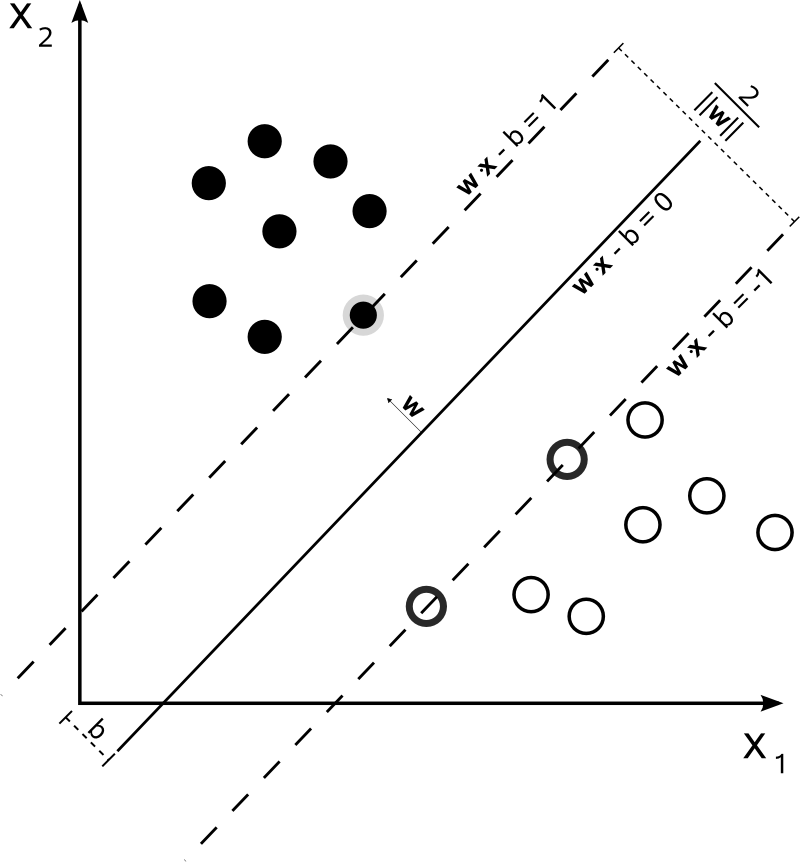
\includegraphics[width=0.4\textwidth]{figures/Svm_max_sep_hyperplane_with_margin}
\end{center}
\caption{{SVM} separating two class of points by a
         \emph{maximal margin hyperplane}. The hyperplane can be described by
         the collection of support vectors and associated weights, marked in the
         image as sample points with large borders.}
\label{fig:svm-sample}
\end{figure}

They have been used in several classification and recognition problems and are
in fact a standard across machine learning techniques. Their efficiency, exact
training results and generalization made them suitable for many tasks. Such as
text categorization, digit-recognition, spam-classification.
They have also been extensively used in visual place classification.
% TODO: add citations.

\subsection{Kernel-Trick}
\label{sec:kernel-trick}
Several classifiers can be modelled by requiring only the concept of inner\hyp{}product
between two samples. That product is often seen as a measure of distance or similarity
between the samples on some space. By using kernels it becomes possible to define such
space without explicit convert the samples to it. By abstracting the concept of distance
on such a kernel function it also becomes possible to use those classification methods
on strange data structures such as trees, strings or graphs.

For example \glspl{SVM}, in their basic form, are only able to handle linear spaces.
But the classes are most of the time not linearly separable in the input
space. Although there might exists a transformation $\phi$ from the original
space into a space $H$ where the input becomes linearly separable.

The Kernel trick allows to extend the \gls{SVM} definition to work on such space
$H$ without ever performing an implicit transformation between spaces. Being
enough for that to have a Kernel function defining an inner-product inside such
space: $K(x_i, x_j) = \phi(x_i)\cdot\phi(x_j)$.

Several kernel functions have been proposed being the most commonly used:

\begin{description}
\item[Polynomial Kernel] - $K(x, y) = (x \cdot y + p)^d$
\item[Radial Basis Function] - $K(x, y) = e^{-\gamma\|x - y \|^2}$
\item[Histogram Intersection] - $K(x, y) = e^{-\gamma \chi^2(x,y)}$, where
$\chi^2(x,y) = \sum_{i=1}^{N}\frac{(x_i-y_i)}{x_i+y_i}$ introduced by
\cite{barla2003histogram} allows to compute histogram similarity.
\item[Matching Kernels] - mimic matching similarity and are used when each
sample is represented as a set of features~\citep{boughorbel2005intermediate}.
\end{description}


\section{Features}
A feature is a piece of information which is expected to reveal information for
solving a specific task. Features are task-dependant and they will
yield different performance based on the type of task they are applied to.

A wanted property on features is its repeatability under similar conditions for
the problem in hand. This is: they should be stable and invariant across
unwanted types of transformations and noise. For example a visual feature for
object detection should be present even if the target object was translated,
scaled, rotated, the light-conditions have changed or even if the object is
partially occluded.

Extracting features with those properties allows to greatly reduce the size of
input by removing unwanted noise and useless information from the captured data.
Turning the classification problem easier, more reliable and more efficient.

Often several and different types of features need to be extracted. It has been
reported by \cite{pronobis2010ijrr} that using multiple features provides a
great benefit in the context of place classification.
And \cite{quattoni2009recognizing} has showed that different types have
different impact in indoor scene recognition based on the type of scene
matching. Specifically it was seen that some room-categories are more likely to be
recognized by the presence of some objects and others by it generic appearance.

In the context of robotics, sensors such as cameras, laser scans are used to
sense the surrounding environment, and features can be extracted from those.
Visual features can be seen as belonging to two categories:
\emph{local features} and \emph{global features}.


\subsection{Local Features}
\label{sec:local-features}
Local features describe fine grain properties of a part of image.
For example the existence of specific corner or an edge. \Gls{SIFT}
is an example of such feature and it been proven useful
for matching points between images and subsequence extension to object detection.

\subsubsection*{Interesting Points and SIFT}
\label{sec:sift}
The detection of interesting points has been studied for several years and is
the base of several computer vision problems solution. It allows to perform
point matching which can be used in several areas from image stitching,
3D reconstruction, video tracking, object detection, etc\dots

The most used method was presented by \cite{lowe1999object}. And its based on
building a feature vector for each image. Each of those features is based on
\emph{interesting points} detected by detecting maxima and minima of a
difference of Gaussian functions applied in a scale-space.
The scale space is used to provide scale invariant detection. Gaussian functions
are used as they are the only way to model a linear scale-space.
Each interesting point is then described by a container that is rotation
invariant.

By seeing an object as a set of features points, index and matching is then
performed by a high-dimensional search on a database of know objects. After
matching objects can be verified for geometric coherence between features.
\Gls{SVM} classifiers can also be trained to detect objects based on this type
of local features by using \emph{Matching kernels} (\autoref{sec:kernel-trick}).

\begin{figure}[h]
    \centering
    
\includegraphics[width=0.8\textwidth]{figures/sift/sift.pdf}
    \caption{{SIFT} and other local features have been proven useful in object
             detection.}
\end{figure}


\subsection{Global Features}
Global features try to describe the whole image. E.g.\ either by
statistical analysis of features over all the image or by a structured
distribution of textures findable in the image.

\subsubsection*{Gist of a Scene}
\label{sec:gist}
\cite{oliva2006building} argue that fast scene recognition does not need to be
built on top of object recognition but can be analyzed by scene-centered
mechanisms.
They defend that position by pointing out behaviours on human vision:
when provided with a glance of a shot a person can identify the meaning of that
given shot or "gist of a scene" without remembering specific details.

As seen on \autoref{fig:gist} the gist is able to capture the dominant textural
features of the overall image and their coarse spatial layout~\citep{murphy2006object}.
With that, it is expected they serve the purpose of correctly describe the image
textures without the need to directly stored the original image.

\begin{figure}[h]
\center
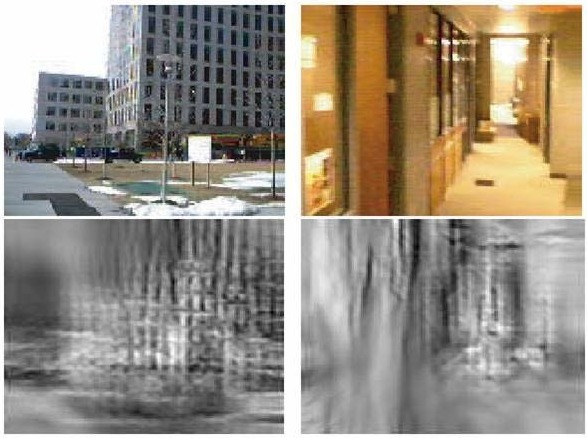
\includegraphics[width=0.60\textwidth]{figures/gist.jpg}
\caption{\label{fig:gist}An illustration of the gist of an image. Top row: original image I;
         bottom row: noise image J for which gist(I) = gist(J).}
\end{figure}


\subsubsection*{{CRFH} - Composed Receptive Field Histograms}
\label{sec:crfh}\label{sec:global-features}
\gls{CRFH} are a multidimensional statistical
representation of the occurrence of several image descriptors applied to an
image. They can be seen as an high-dimension histogram where each cell records
how many pixels of the image have the cell response for the applied descriptors.
Such high-dimensional histogram is expected to be able to describe global
information contained in the image by capturing several properties that co-occur
in a part of the image.
By using some techniques~\cite{linde2004object} several operations on those
high-dimensional histograms can be made computational efficient. This way not
only this descriptor discards part of the local information present on the image
but also allows to faster computations on similarity measures.


\begin{figure}[h]
\begin{center}
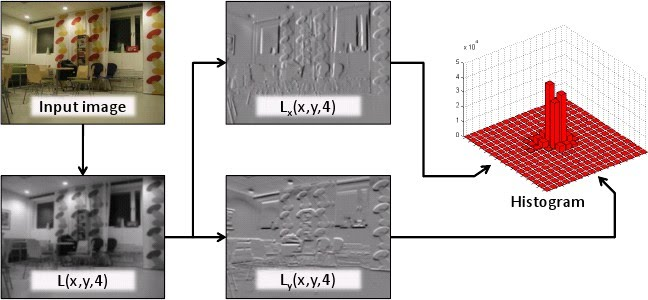
\includegraphics[width=1\textwidth]{figures/crfh_model.jpg}
\end{center}
\caption{A two dimensional histogram of the image built out from two image
         descriptors: $Lx$ and $Ly$. First-order Gaussian derivatives of image
         luminance in horizontal and vertical direction applied at a scale 4.}
\end{figure}

Multidimensional histograms have proven to be useful in the context of object
recognition~\citep{schiele1996object}. And have also been previously used in
the context of visual place classification~\cite{pronobis2010ijrr}.
\emph{Histogram intersection kernels} (\autoref{sec:kernel-trick}) can be used
to train classifiers based on this feature.


%%%%%%%%%%%%%%%%%%%%%%%%%%%%%%%%%%%%%%%%%%%%%%%%%%
% Important sections of this chapter begin here.
%%%%%%%%%%%%%%%%%%%%%%%%%%%%%%%%%%%%%%%%%%%%%%%%%%
\section{Probability Theory}
An important aspect when making decisions with noisy or missing information is
the uncertainty of the received information and of the final conclusion.
Probability theory comes to help by providing a framework able to deal with those
issues~\cite{bishop2006pattern}.

The key concept on it is that of \emph{probability}, which can be seen as way of
express the degree of belief that a certain event occurs.
When combined with decision theory it allows to perform optimal decisions with the
available information, even if it is ambiguous or incomplete.

A probability $P(x)$ of a given event $x$ is a value between $0$ and $1$, where $0$ means
the belief that $x$ will not occur and $1$ that it will certainly occur.
In cases $x$ does not specifies all the variables states that define the sample space, $P(x)$
is called a marginal probability. 

Often it is impossible to exactly describe the probability of a given event, in such cases
the concept of likelihood comes to help.
The likelihood of an event only has meaning when compared to one of another event.
In such case the ratio between both likelihoods will denote on how more likely an event is
over another.
When dealing with discrete and countable sample spaces any likelihood function can be converted
to a probability function by calculating the normalization factor such that the sum over all
the sample space is $1$.

\subsection{Conditional Probability}
It is also possible to denote the known information when calculating probabilities. For that
the notion of conditional probability is used $P(a|b)$. It denotes the probability of $a$
knowing that $b$ has occur. Often conditional probability is also represented by: $P_b(a)$.
In this thesis both notations will be used: the former for representing the information on
sensed variables and the second for representing information or assumptions on other generic
information such as graph structures.

Marginal probabilities can be related with conditional probabilities as described in the equation:
\begin{equation}
P(a|b) P(b)  = P(a, b)
\end{equation}


\section{Principle of Maximum Entropy}
\label{sec:max-entropy}
The principle of maximum entropy~\cite{shore1980axiomatic} states that when given
a set of distributions that are coherent with the acquired knowledge, the one which
maximizes entropy should be picked.

This can be used to select a distributions that most correctly describes the obtained
knowledge. For example, if all that is known from a distribution is the mean and deviation
then the correct approach is to model it with a normal distribution with the known parameters.
In case of having no information available, the uniform distribution shall be assumed.


\section{Probabilistic Graphical Models}
\label{sec:graphical-models}
% THIS IS ALL JUNK TEXT COPIED
Graphical models usage can be tracked back to earlies 1920 but they only become
popular in mid-eighties when researchers started to use \emph{Bayesian Networks}
to model expert systems~\citep{borgelt2002graphical}.

They serve as a better tool to model \emph{random variables}
(nodes on the graph) and their probabilities as they model the conditional
dependence between variables (edges on the graph). Important to note that here
\emph{random variables} does not denotes a truly random variable but one that is
unknown by the system and is conditioned by other variables/evidences.

This type of graphs provide a generative model where the probability of any
given scenario can be determined.
This means once a graphical model is learned, it can be used to generate new
samples from the learned distribution.

They have been successfully used in several machine-learning task such as:
information extraction, speech recognition, computer vision.
They are also useful due to their ability to deal with semantic (high-level)
features~\citep{boutell2006factor} and ability to represent properties of the
reality they try to model.

Two main types of graphical models are widely used: Bayesian Networks which model
directed edges between variables and Markov Random Fields where variables are
connected by a potential but no special direction is given to edges.

An important property of these graphs is the \emph{Markov-blanket} of a node.
For a given variable $a$, a \emph{Markov-blanket} is a set of variables in the
surroundings of $a$ that when given the value of $a$ becomes independent of the
rest of the graph~\citep{pearl1988probabilistic}.
On non-directional graphs it is directly determined by the nodes connected to $a$.
This allows the usage of graph algorithms such as \emph{min-cut} to quickly
determine most likely scenarios. In the case of directed edges a node blanket is
also influenced by the direction of the edges and more complex schemes need to
be used.

As \cite{lauritzen2002chain} points this two types of models can be represented
as a \emph{chain graph} where both directed and undirected edges can co-exist.
Though this generalization is hard to implement due to mis-understandings on the
concepts the graph-models use.

Another useful interpretation of graphical-models are \emph{factor graphs}.
Those are able to handle both \emph{Bayesian Networks} and
\emph{Markov Random Fields}. Under this interpretation a graph is seen as a
bipartite graph that connects variables with factors that influence
them~\citep{bishop2006pattern}.
This gives a very useful framework to develop belief propagation on them by
seeing a message-passing mechanism between nodes. Belief propagation is used to
calculate marginal-probabilities.

\begin{figure}[ht]
\centering

\subfloat[Bayes Networks] {
  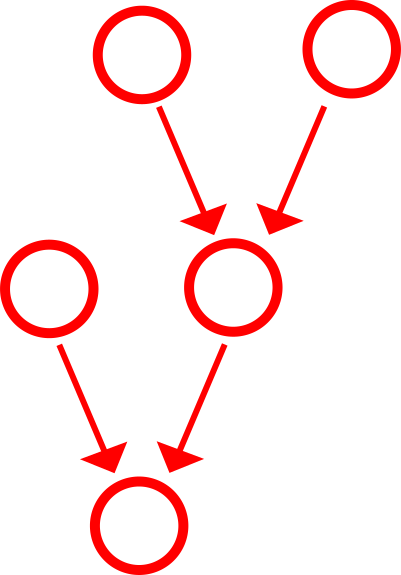
\includegraphics[width=0.2\textwidth]{figures/graphical-models/BayesNet.pdf}
}
\quad
\subfloat[Markov Random Field] {
  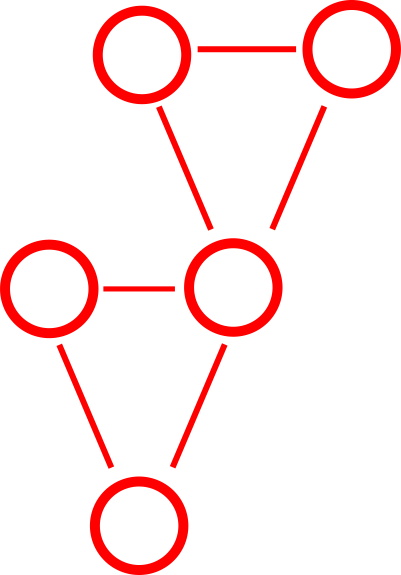
\includegraphics[width=0.2\textwidth]{figures/graphical-models/MarkovRandomField.pdf}
}
\quad
\subfloat[Factor Graph] {
  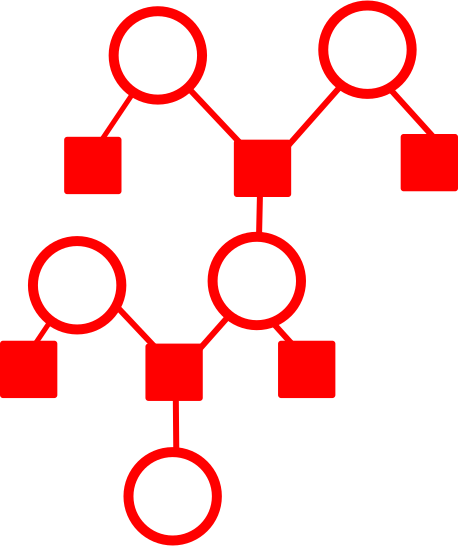
\includegraphics[width=0.3\textwidth]{figures/graphical-models/FactorGraph.pdf}
}
\end{figure}

\subsection{Factor Graphs}
A \emph{factor graph}~\cite{kschischang2001factor} is a bipartite graph connecting two sets of nodes $X_G$ and $F_G$
representing random variables and factors.
Each factor is described by function $\phi$ dependent only on the variables $x_\phi$
to which the factor is connected.
Thus, a factor graph can be seen as a description of probability density function obtained
by a product of all the factors. In order to represent the probability,
a normalization factor needs to be introduced, resulting in the following equation:

\begin{equation}
P_G(x) = \frac{1}{Z}\prod_{\phi \in F_G}{\phi(x_{\phi})},\qquad
Z = \sum_{X_G}\prod_{\phi \in F_G}{\phi(x_{\phi})}
\end{equation}

\subsection{Inference}
The goal by obtaining a graphical model between all the variables of a system is the ability
to efficiently infer the most likely scenarios based on the available information.
The sensed information can be used to clamp variables and the model used to calculate probabilities
or marginal probabilities.

In that sense a basic operation on a graph is the \gls{MAP} operation, which allows to calculate
which configuration on a variable or subset of variables maximizes a given function.

\chapter{Approach}
\label{chap:approach}
In this chapter an overview of the approach used to address the problem of place classification in mobile robotics and concerns regarding implementing novelty detection on it are presented.


\section{Overview}
Graphical models have shown to be useful as they allow to unify the whole set of beliefs that influence a given variable, which is expected to lead to better results than exploiting a single source of information (\autoref{sec:related-work}).

Our approach is based on a \emph{chain graph} representation that combines general purpose knowledge with spatial knowledge and uses probabilistic perception to model variables.

Using a map of the environment or other knowledge (for example given by a user) the graph is built with the variables that the system wants to model (rooms, objects, sensed perceptions).
Connectivity between those variables is then created using default knowledge: such as probabilities of room connectivity or object existence on a given room category.
The low-level sensors are passed through classifiers and their results are plugged into the model.

Using that \emph{graph} the robot can then perform inferences on the variables and estimate the most likely scenario. 
It can be used for example to query about specific variables: that a given room is a kitchen.
Or used to perform high-level reasoning operations such as strategy-planning.


\section{Layers}
The system can be decomposed in four layers:
\emph{Conceptual Layer}, \emph{Categorical Layer}, \emph{Place Layer} and \emph{Sensory Layer}.
Each of them will be presented to the reader in the next sections starting from the high-level \emph{Conceptual Layer} and diving depth into the low-level ones.
\autoref{fig:system-structure} shows the 4 layers and draws lines related to their interaction. A look at the figure with a simultaneous reading of the layers is encouraged.

Special interest for novelty detection and place classification is on the \emph{Conceptual} and \emph{Categorical Layer} as they are the ones responsible for probabilistic modeling and classification.


\subsection{Conceptual Layer}
% TODO graphics:
% World <--> | wall | <--> sensors <--> Graphical model
While the robot moves through the environ it builds a graphical model (\autoref{sec:graphical-models}).
That graph models and relates the unknown variables that the robot tries to extract from reality.
The connections between those random variables can be seen as a filter of possible probability distributions for them \citep{bishop2006pattern}. It is therefore important the way the graph is connected and which variables it models since that is the world model the robot is using.

The description of the modeled variables and factors is given on the next subsections.
\subsubsection*{Modelled Variables}
\begin{description}
\item[Room Category] represents the category the room belongs to. This is the variable used as output to the the place classification.
\item[Room Shape] represents the type of room shape, such as elongated, square. The output of the laser scan is used to condition this variable.
\item[Room Appearance] represents what the room \emph{looks like}, this is associated with the global visual feature classifier.
\item[Object Presence] represents a given object. This variable is conditioned by the object detector which uses local visual features.
\end{description}

\subsubsection*{Modelled Factors}
\begin{description}
\item[Room-Room Connectivity] models the probability that two given rooms are connected. For example class rooms are very likely to be connected to a corridor.
\item[Room-Object Connectivity] models the object presence in a given room.
\item[Observed Room Shape] models the sensed room shape by the classification layer.
\item[Observed Room Appearance] models the sensed room appearance by the classification layer.
\end{description}


\subsection{Categorical Layer}
This layer is responsible from extracting properties from the sensors.
It has classifiers trained to detect several properties from the visual and laser data captured from the robot sensors.

So far the following properties are extracted:
\begin{description}
\item[Object presence] using \emph{local visual features} (\autoref{sec:local-features}).
\item[Place appearance] using \emph{global visual features} (\autoref{sec:global-features}).
\item[Room shape and size] using \emph{geometric features} from 2D laser data to classify properties as: square/elongated and room size.
\item[Landmark detection] uses 2D laser data to detect doors.
\end{description}


\subsection{Place Layer}
The place layer is responsible for the low-level movement and mapping of the environment.
The robot spreads several virtual places markers around the whole environment and maintains connectivity information between them.

By using the door landmarks detected by the categorical layer, it becomes then possible to group the place markers to create the concept of room.

Also this low-level places together with information associating the robot view point with extracted properties allows the system to perform a clever integration over the room properties, avoiding sampling bias, for example coming due to the robot spend too much time in a part of the room (\autoref{sec:accumulation}).

\subsection{Sensory Layer}
This layer captures data from the robots sensors, those include images from cameras, 2D laser scans and odometry from encoders in the movement motors.


\begin{figure}[h]
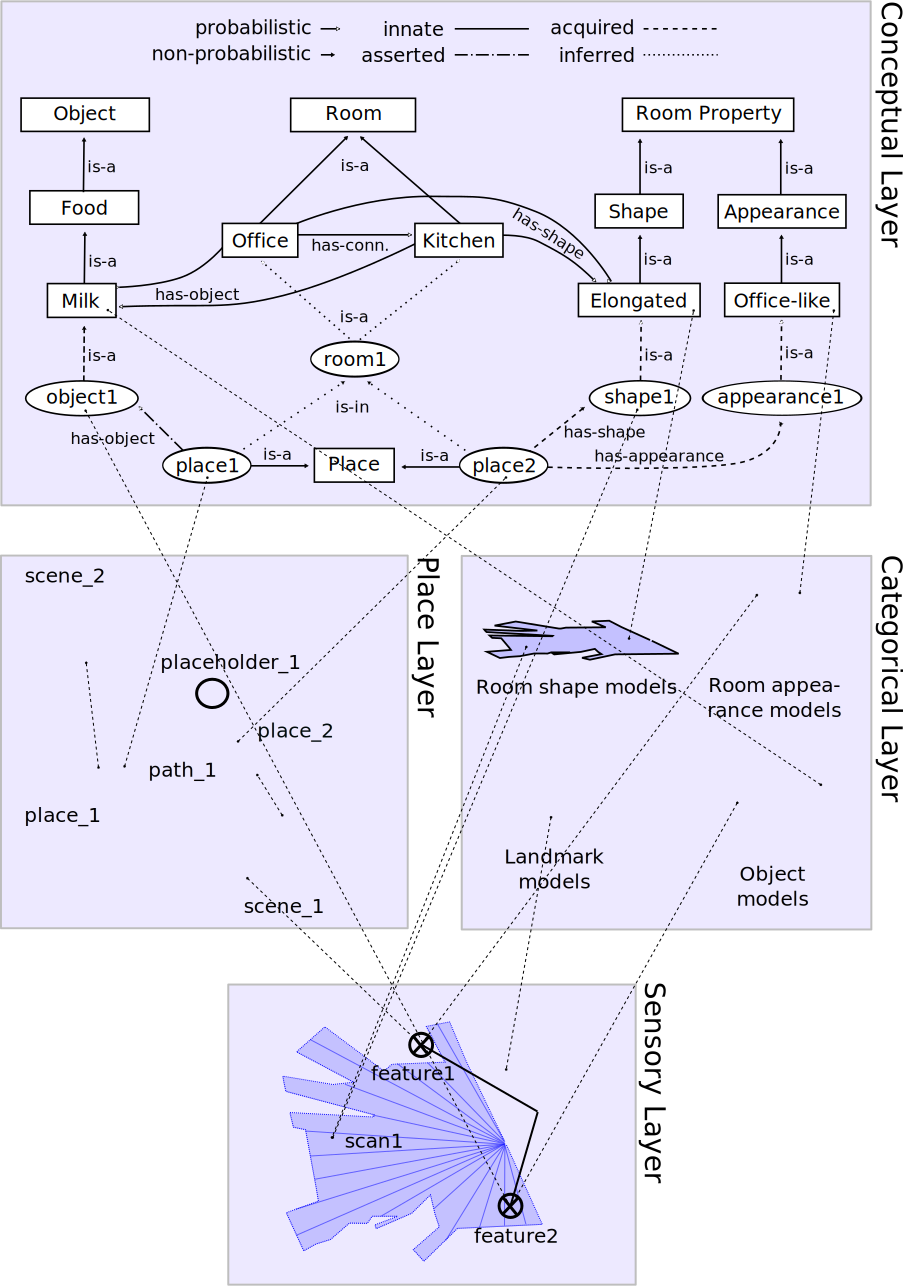
\includegraphics[width=\textwidth]{system-representation/structure}
\caption{In the figure its possible to visualize the interactions of the 4 layers that composed the proposed approach. Novelty detection will have special impact on the \emph{Conceptual} and \emph{Categorical Layers},}
\label{fig:system-structure}
\end{figure}



\section{Novelty Detection}
\label{sec:approach-novelty}
In the previous sections the used approach for the problem of visual place classification was presented.
That system has been used with success by \cite{pronobis2011exploiting} and has demonstrated to be efficient for planning and high-level reasoning under dynamic ambients.

Nonetheless the system has no knowledge about novelty and when presented with a classification task it has to classify the room into one of the room classes it knows.
This poses problems and performance decrease when the robot is deploying into new environments where the room categories or other world variables are novel to the system.

The inability of the robot to handle novel cases (a room which belongs to a category the system was not trained with) is translated at the graphical model not being prepared to handle a unknown variable value.
The detection of novel values (\autoref{sec:novelty-detection}) can be done by triggering on the unconditional probability density for the given input.
Since the presented approach uses a \emph{generative model} we expect such an approach to be feasible.

At a lower-level the system also needs to be extended to handle novelty at the classifiers used to extract properties. In that case novel inputs from the sensors translate as the inability for the classifier to operate correctly and so less confidence must be given to its results. That 
Those classifiers after training do not provide a \emph{generative models} rendering a probabilistic estimation approach infeasible.
For that case other approaches such as \gls{K-PCA} (\autoref{sec:kernel-pca}) will be used to address the problem.


\chapter{Datasets and Evaluation}
\label{chap:testing}
This chapter describes the methods and databases used to gather data and evaluate the developed work. It also presents the \gls{ImageCLEF} competition to which the work will be submitted to.

\section{Common Sense Databases}
There are several databases that can be used to represent common sense for human reasonning.
From those databases several probabilistic relations can be derived in order to increase the quality of the model the robot uses for reasoning at high-level.
Examples of those databases are:

{OpenMind Common Sense}~\citep{singh2010open} which contains several sentence-templates filled in by humans by creating meaningful sentences (\autoref{fig:openmind-sample}). With those its possible to extract knowledge of finding certain objects in room categories.

\begin{figure}[!h]
\centering
\fbox{
\begin{minipage}{13 cm}
A kitchen floor is dirty when a kitchen floor is sticky.\\
A room where you generally find a muffin is the kitchen.\\
You generally find a blender in a kitchen.\\
An object that you might find in an office is a answering machine.\\
An object that you might find in an office is a briefcase.
\end{minipage}
}
\caption{Examples of sentences available on OpenMind Indoor Common Sense}
\label{fig:openmind-sample}
\end{figure}


\begin{figure}[!h]
\begin{center}
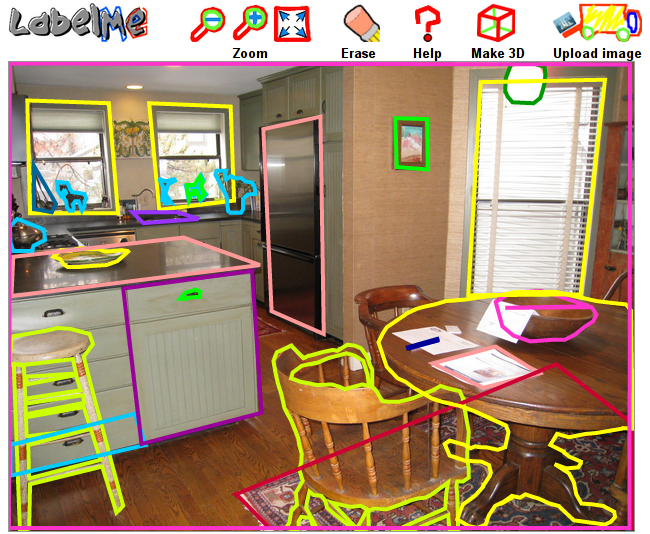
\includegraphics[width=0.7\textwidth]{labelme_kitchen_sample}
\end{center}
\caption{Sample annotated image from the LabelMe online database.}
\label{fig:labelme_sample}
\end{figure}

LabelMe~\citep{russell2008labelme} which is an online database for image annotation (\autoref{fig:labelme_sample}.
At the moment it counts with hundreds of thousands labelled objects.
There is both images and sequences of images that have been annotated.
The annotation does not only goes for objects but also for scene categories,
turning this database useful for extraction of data related with probabilities of finding objects in room categories. As well their appearance.

\section{Evaluation Databases}\label{sec:databases}
In order to train and evaluate the system real databases are required. In that sense we point to a previously used database: \gls{COLD}~\citep{pronobis09ijrr-cold}.

It contains image sequences captured using a regular and omni-directional cameras together with laser range scans and odometry data.
The data were recorded using three different mobile robot platforms and the same camera setup, under various weather and illumination conditions (during cloudy weather, sunny weather and at night) over several days.
In each of the three labs, the acquisition was performed in several rooms of different functionality.


\begin{figure}[!h]
\label{fig:cold-database-sample}
\begin{center}
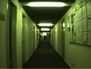
\includegraphics[width=0.15\textwidth]{cold/Saarbruecken_CR}
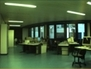
\includegraphics[width=0.15\textwidth]{cold/Saarbruecken_TR}
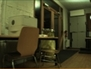
\includegraphics[width=0.15\textwidth]{cold/Freiburg_PA}
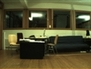
\includegraphics[width=0.15\textwidth]{cold/Freiburg_LO}
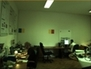
\includegraphics[width=0.15\textwidth]{cold/Ljubljana_LAB}
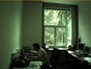
\includegraphics[width=0.15\textwidth]{cold/Ljubljana_2PO}

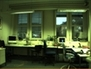
\includegraphics[width=0.15\textwidth]{cold/Saarbruecken_RL}
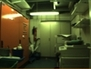
\includegraphics[width=0.15\textwidth]{cold/Saarbruecken_PA}
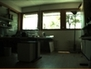
\includegraphics[width=0.15\textwidth]{cold/Freiburg_1PO}
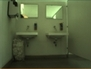
\includegraphics[width=0.15\textwidth]{cold/Freiburg_TL}
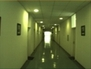
\includegraphics[width=0.15\textwidth]{cold/Ljubljana_CR}
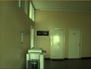
\includegraphics[width=0.15\textwidth]{cold/Ljubljana_PA}

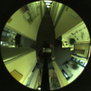
\includegraphics[width=0.15\textwidth]{cold/Saarbruecken_CR(1)}
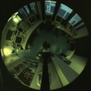
\includegraphics[width=0.15\textwidth]{cold/Saarbruecken_TR(1)}
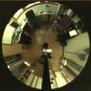
\includegraphics[width=0.15\textwidth]{cold/Freiburg_1PO(1)}
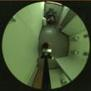
\includegraphics[width=0.15\textwidth]{cold/Freiburg_TL(1)}
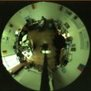
\includegraphics[width=0.15\textwidth]{cold/Ljubljana_LAB(1)}
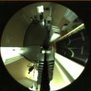
\includegraphics[width=0.15\textwidth]{cold/Ljubljana_PA(1)}
\end{center}
\caption{Sample data from the COLD database. Images were acquired from three diferent indoor laboratory enviroments located in diferent European cities: Saarbrücken, Freiburg and Ljubjlana.}
\end{figure}



Consequently, the \gls{COLD} database is an ideal testbed for assessing the robustness of localization and place recognition/categorization algorithms with respect to both categorical and dynamic changes (introduced by illumination variations and human activity).

The \gls{COLD} database is also in the process of being extend with additional data from Stockholm labs in \gls{KTH}.


\section{{ImageCLEF} - Robot Vision Task}
\subsection{History}
\gls{ImageCLEF} is the cross-language image retrieval track which is run as part of the Cross Language Evaluation Forum (CLEF). \gls{ImageCLEF} has already seen participation from both academic and commercial research groups worldwide from communities~\citep{imageclef}.
Together with each task run, datasets of training and validation data are made available providing the community with useful tools for benchmarking their methods.

It exists since 2003 and the tasks proposed by it have been evolving over-time and in 2010 it counted four main tasks: Medical Retrieval, Photo Annotation, Robot Vision and Wikipedia Retrieval.
Of which the Robot Vision is of interest to this thesis.


\subsection{Robot Vision Task in 2011}
The robot vision task~\citep{pronobis2010imageclef} which originally has been part of the \gls{ImageCLEF} since 2009 will no longer be part of it.
Nonetheless according to the organizers the competition will keep its structure and will remain active as a sole competition not part of the forum.

A transcription of the challenge description follows:

\begin{quotation}``The third edition of the challenge (2011) will focus on the problem of visual place classification, with a special focus on generalization.
Participants will be asked to classify rooms and functional areas on the basis of image sequences, captured by a stereo camera mounted on a mobile robot within an office environment.
The test sequence will be acquired within the same building but at a different floor than the training sequence.
It will contain rooms of the same categorical type ("corridor", "office", "bathroom") and it will also contain room categories not seen in the training sequence ("meeting room", "library").

The system built by participants should be able to answer the question "where are you?" when presented with a test sequence imaging a room category seen during training, and it should be able to answer "I do not know this category" when presented with a new room category.'' -- Robot Vision Task
\end{quotation}


\chapter{Work Plan}
\label{chap:workplan}
In order to accomplish the goals described in \autoref{sec:goals} several work needs to be done.
This chapter presents the several task under which the work has been split into.
Those cover the basic literature review and study, developing, testing, evaluation and writing the final report and presentation of this thesis.

\section{Tasks Description}
\subsection{Literature Review}
Although during the preparation of this report several concepts and theories were already studied, during the thesis they will need to be deeper analysed and studied.
This task is expected to be spread out during the whole thesis preparation though with a bigger impact in the beginning.

\subsection{Study Property-base semantic mapping system}
Adding to the base literature review, the novel proposed system \cite{pronobis2011exploiting} requires additional study and understanding as one of the focus of this thesis is the evaluation of that system. This will be one of the first tasks to be completed.

\subsection{Implement novelty detection algorithms}
As described in \autoref{sec:approach-novelty} novelty detection can be seen as two separate methods.
Those two methods will be implemented, starting with the identification of novel room types directly on the \emph{graphical model}.
Later the graphical model will be expanded to be able to handle novelty signals from the classifiers used to extract sensed properties.

\subsection{Testing and Evaluation of developed methods}
A step of this thesis is an evaluation of the used approach and determination of its efficiency.
The developed methods will be run through the databases described in \autoref{sec:databases}.

The results will be compared and used for tunning parameters and redirect research efforts.
For final evaluation and comparison the developed method will be submitted to robot task of \gls{ImageCLEF}.

\subsection{Thesis Writing}
As final stage all the study and results will be written in the Master thesis and its presentation will be prepared.

\section{Tasks Schedule}
Due to the nature of the tasks at hand its impossible to predict exact dates or give precise and detailed description on each of them.

We point to the fact that novelty research on itself is not an easy topic as it requires specific knowledge to each case. And also the approaches detailed here are novel on itself and its impossible to predict the problems that may appear as we move forward on the research.

Its however possible to give an high-level level overview of the tasks and their order of execution.
As presented on the graph below:
\begin{figure}[!h]
\center
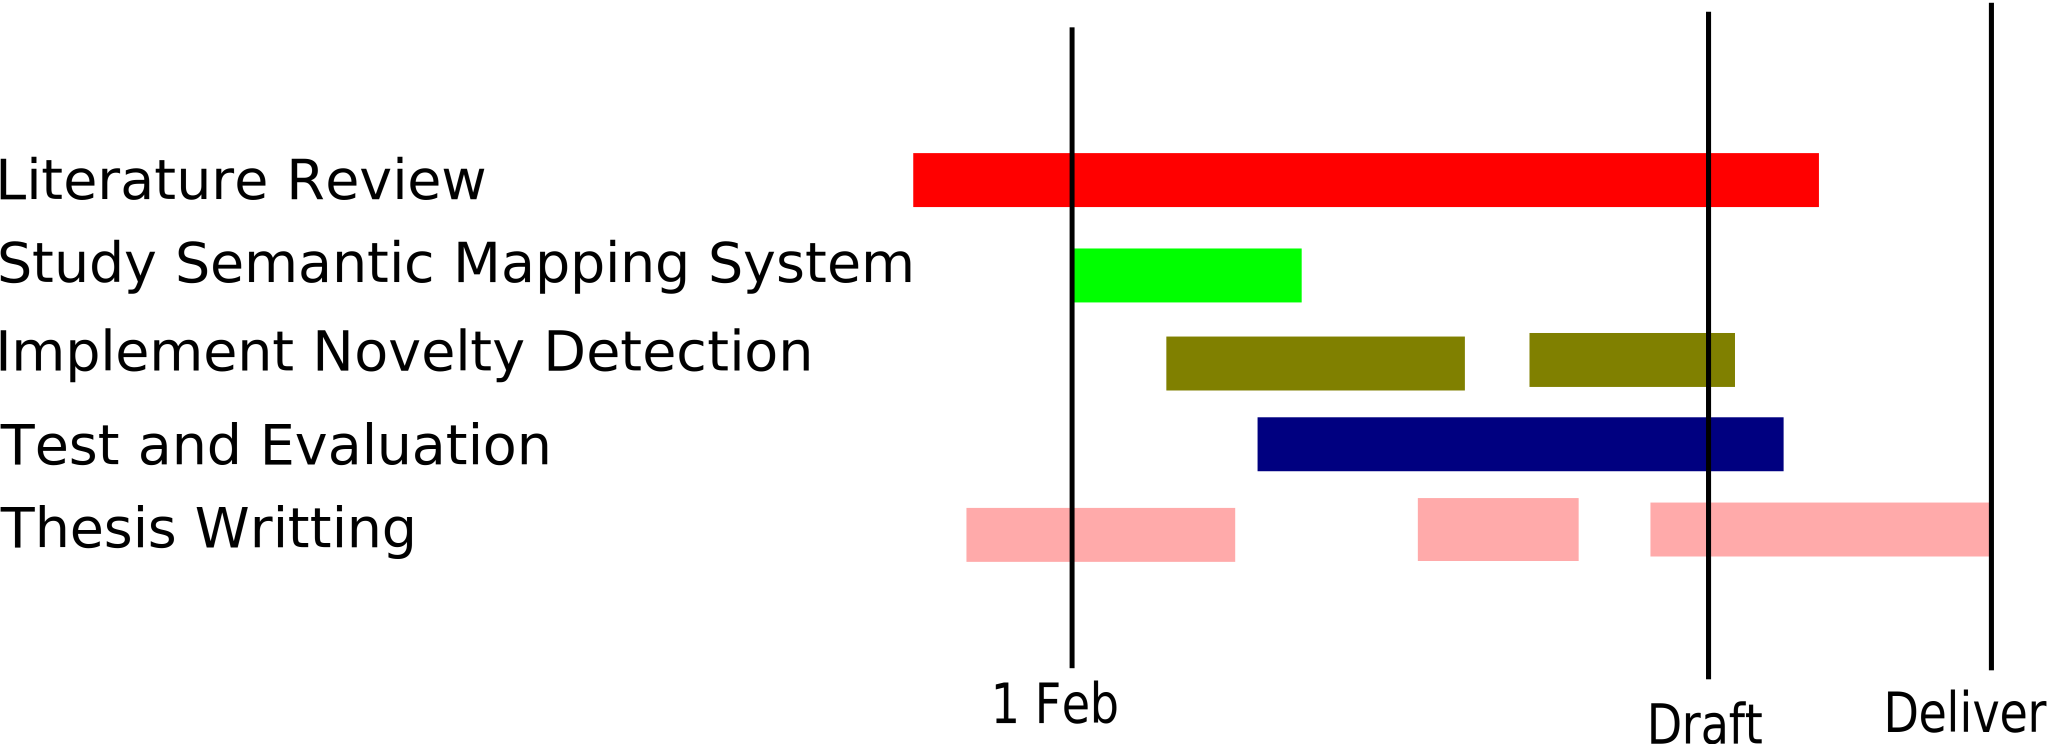
\includegraphics[width=\linewidth]{gantt.pdf}
\caption{Scheme of tasks to be completed over time.}
\end{figure}

As shown the literature review, thesis writing and a small part of the system study were the main focus until the moment. Since that was required knowledge to the writing this report.

Next focus will be on implementation of novelty detection on top off the graphical-model. Test and evaluation also start earlier as scripts and performance measures need to be established in order to correctly implement the developed methods. Some writing will be involved after that in order to report results on the developed method.

After that focus will be on integration of novelty detection at the level of properties classifiers. And respective changes on the graphical-model to handle that additional information provided by the classifiers.

At last efforts will be redirected to the conclusion of the thesis writing and preparation of its presentation.

 

%%----------------------------------------
%% Final materials
%%----------------------------------------

\begin{singlespace}
  %% Bibliography
  %% Comment the next command if BibTeX file not used, 
  %% bibliography is in ``myrefs.bib''
  % \PrintBib{refs}

  % SCons build system does not recognized the bibliography
  % if its nested inside this templates and new commands of
  % feup-teses.
  % For that reason instead of using \PrintBib{Refs}
  % the contents of that command is pasted here.
  \renewcommand{\bibname}{References}%
  \bibliographystyle{plainnat}%
  \cleardoublepage%
  \phantomsection%
  \addcontentsline{toc}{chapter}{References}%
  \bibliography{myrefs}

  %% Index
  %% Uncomment next command if index is required,
  %% don't forget to run ``makeindex mieic'' command
  %\PrintIndex

  %% Comment next 2 commands if numbered appendixes not used
  %\appendix
  %\chapter{Loren Ipsum} \label{ap1:loren}

Depois das conclusões e antes das referências bibliográficas,
apresenta-se neste anexo numerado o texto usado para preencher a
dissertação.

\section{O que é o \emph{Loren Ipsum}?}

\emph{\textbf{Lorem Ipsum}} is simply dummy text of the printing and
typesetting industry. Lorem Ipsum has been the industry's standard
dummy text ever since the 1500s, when an unknown printer took a galley
of type and scrambled it to make a type specimen book. It has survived
not only five centuries, but also the leap into electronic
typesetting, remaining essentially unchanged. It was popularised in
the 1960s with the release of Letraset sheets containing Lorem Ipsum
passages, and more recently with desktop publishing software like
Aldus PageMaker including versions of Lorem Ipsum~\citep{kn:Lip08}. 

\section{De onde Vem o Loren?}

Contrary to popular belief, Lorem Ipsum is not simply random text. It
has roots in a piece of classical Latin literature from 45 BC, making
it over 2000 years old. Richard McClintock, a Latin professor at
Hampden-Sydney College in Virginia, looked up one of the more obscure
Latin words, consectetur, from a Lorem Ipsum passage, and going
through the cites of the word in classical literature, discovered the
undoubtable source. Lorem Ipsum comes from sections 1.10.32 and
1.10.33 of ``de Finibus Bonorum et Malorum'' (The Extremes of Good and
Evil) by Cicero, written in 45 BC. This book is a treatise on the
theory of ethics, very popular during the Renaissance. The first line
of Lorem Ipsum, ``Lorem ipsum dolor sit amet\ldots'', comes from a line in
section 1.10.32.

The standard chunk of Lorem Ipsum used since the 1500s is reproduced
below for those interested. Sections 1.10.32 and 1.10.33 from ``de
Finibus Bonorum et Malorum'' by Cicero are also reproduced in their
exact original form, accompanied by English versions from the 1914
translation by H. Rackham.

\section{Porque se usa o Loren?}

It is a long established fact that a reader will be distracted by the
readable content of a page when looking at its layout. The point of
using Lorem Ipsum is that it has a more-or-less normal distribution of
letters, as opposed to using ``Content here, content here'', making it
look like readable English. Many desktop publishing packages and web
page editors now use Lorem Ipsum as their default model text, and a
search for ``lorem ipsum'' will uncover many web sites still in their
infancy. Various versions have evolved over the years, sometimes by
accident, sometimes on purpose (injected humour and the like). 

\section{Onde se Podem Encontrar Exemplos?}

There are many variations of passages of Lorem Ipsum available, but
the majority have suffered alteration in some form, by injected
humour, or randomised words which don't look even slightly
believable. If you are going to use a passage of Lorem Ipsum, you need
to be sure there isn't anything embarrassing hidden in the middle of
text. All the Lorem Ipsum generators on the Internet tend to repeat
predefined chunks as necessary, making this the first true generator
on the Internet. It uses a dictionary of over 200 Latin words,
combined with a handful of model sentence structures, to generate
Lorem Ipsum which looks reasonable. The generated Lorem Ipsum is
therefore always free from repetition, injected humour, or
non-characteristic words etc. 

\end{singlespace}

\end{document}
